\documentclass[conference]{IEEEtran}
\IEEEoverridecommandlockouts

\usepackage[utf8]{inputenc}
\usepackage[T1]{fontenc}
\usepackage[spanish]{babel}
\usepackage{graphicx}
\usepackage{booktabs}
\usepackage{amsmath}
\usepackage{url}
\usepackage{hyperref}

\addto\captionsspanish{\renewcommand{\tablename}{Tabla}\renewcommand{\figurename}{Fig.}}
\hypersetup{hidelinks}
\renewcommand{\IEEEkeywordsname}{Palabras clave}
\def\UrlBreaks{\do\/\do-\do.\do:\do\_\do=\do?\do&\do\%\do\#}
\Urlmuskip=0mu plus 2mu
\emergencystretch=1.5em

\title{Perfiles multidimensionales de brecha tecnológica en los locales educativos del Perú: recursos, conectividad y cobertura móvil territorial}

\author{
\IEEEauthorblockN{Francisco Luis Delgado Santana, Nicole Rashel Pando Cabezas, Brayan Anderson Rua Pomahuacre}
\IEEEauthorblockA{Grupo: Mineros \\
Curso: Data Mining \\
Universidad del Pacífico \\
Docente: Soledad Espezúa Llerena}
}

\begin{document}
\maketitle

\begin{abstract}
La brecha tecnológica de los locales educativos del Perú combina conectividad, equipamiento y cobertura móvil, y saber si un local tiene internet no basta para distinguir sus necesidades. Este avance busca perfiles de brecha en 42\,215 locales, con datos del MINEDU (ESCALE) y del OSIPTEL. Los 17 indicadores se transforman (\texttt{log1p}, estandarización) y se resumen en cinco componentes principales (84,4~\% de la varianza). Se comparan K-means (k de 2 a 8), Ward y DBSCAN con silueta y Davies-Bouldin; se elige K-means con k = 5 (silueta 0,331; Davies-Bouldin 1,073), mientras que DBSCAN no produce perfiles útiles. Los perfiles van desde locales conectados con cobertura 4G/5G (16,8~\%) hasta locales pequeños y desconectados (31,4~\%), y su distribución territorial difiere entre departamentos. Quedan pendientes la validación con área y gestión y la detección de anomalías.
\end{abstract}

\begin{IEEEkeywords}
clustering, K-means, PCA, brecha tecnológica, locales educativos
\end{IEEEkeywords}

\section{Introducción}
La brecha tecnológica de los locales educativos del Perú no se reduce a tener o no internet. Un local puede estar conectado y tener equipos que necesitan reparación; otro puede contar con equipos y carecer de conexión, y todos están en entornos con distinta cobertura móvil. Saber solo si hay internet deja sin explicar estas combinaciones.

El análisis se dirige al Ministerio de Educación (MINEDU), las Direcciones Regionales de Educación (DRE) y las Unidades de Gestión Educativa Local (UGEL), que podrían reconocer necesidades distintas de conectividad, equipamiento y mantenimiento.

El objetivo es identificar, mediante clustering, perfiles de brecha tecnológica en los locales educativos del Perú, considerando su acceso a internet, la disponibilidad y el estado de sus recursos tecnológicos y la cobertura móvil de su entorno. La \textbf{pregunta de análisis} es: ¿qué perfiles de brecha tecnológica se distinguen entre los locales educativos del Perú al combinar estas tres dimensiones, y cómo se distribuyen en el territorio? La detección de casos atípicos, también prevista en el Hito 2, queda para el Hito 4.

Código y cuaderno: \url{https://github.com/franciscosdafas133/Data_Mining_Project/tree/hito3}.

\section{Datos y representación final}
\textbf{Fuentes y unidad.} Se usan cuatro bases del Censo Educativo 2025 del MINEDU (portal ESCALE): ficha lineal del local, recursos tecnológicos (P91), líneas de internet (P3230) y padrón de locales (Padlocal) \cite{escale}. A ellas se suma la cobertura móvil por centro poblado, operadora y tecnología del OSIPTEL (2025-IV) \cite{osiptel}, resumida por distrito. La unidad de análisis es el local educativo.

\textbf{Integración.} La información del MINEDU se une por código de local (censo con recursos mediante unión interna; después, líneas y padrón por unión izquierda) y la cobertura, por código de distrito. Resultan 42\,221 locales. Los otros 24\,924 de los 67\,145 locales del censo quedan fuera por no tener registro de recursos, de modo que los resultados describen solo los locales incluidos.

\textbf{Variables.} La matriz analítica tiene 17 variables: cantidad total de recursos; proporción de recursos operativos, en reparación y operativos con más de tres años (sobre el total); presencia de cuatro familias de recursos (cómputo, infraestructura TI, multimedia y periféricos, tablets y móviles); internet del local, internet del centro poblado y número de líneas; y seis indicadores de cobertura móvil distrital (4G y 5G: promedio, mejor cobertura entre operadoras y proporción de centros poblados cubiertos). No entran identificadores, nombres geográficos ni coordenadas (sirven para interpretar), velocidades y ancho de banda (muchos faltantes), financiamiento, ni área y gestión, que se reservan para validar los grupos.

\textbf{Transformaciones.} Se excluyen los 6 locales con algún faltante (uno con inventario dudoso marcado como faltante y cinco sin cobertura distrital), con lo que la matriz queda en 42\,215 $\times$ 17. Se aplica \texttt{log1p} a las dos cantidades (recursos y líneas) y \texttt{StandardScaler} a las 11 variables no binarias; las 6 binarias se mantienen en 0/1, de modo que sus promedios se leen como porcentajes. Esto reemplaza el escalamiento Min-Max del Hito 2. Los valores extremos se conservan. Sobre la matriz se aplica PCA y se retienen cinco componentes ($Z_1$--$Z_5$), que suman 84,4~\% de la varianza (cuatro llegan a 78,7~\%) y forman la matriz $Z_{df}$ de 42\,215 $\times$ 5. $Z_1$ (46,7~\%) reúne los seis indicadores de cobertura, con pesos entre 0,36 y 0,41.

\section{Metodología}
La técnica es clustering no supervisado: no hay variable objetivo y se buscan grupos de locales con condiciones similares. Se usa K-means \cite{lloyd} sobre $Z_{df}$, porque se aplica a los 42\,215 locales, asigna cada uno a un solo grupo y permite describir cada perfil con los promedios de las variables originales. El PCA \cite{jolliffe} precede al clustering para trabajar con menos dimensiones y sin correlación entre ellas. Como contraste se aplican Ward \cite{ward} (jerárquico) y DBSCAN \cite{ester} (por densidad, sin fijar el número de grupos). La implementación usa Python con scikit-learn \cite{sklearn}.

K-means supone grupos compactos y usa distancia euclidiana, por lo que el resultado depende de la estandarización y del PCA. Además, la cobertura móvil es distrital y pesa mucho en $Z_1$.

Para la lectura territorial, cada local se ubica en una provincia mediante unión espacial con la capa de provincias del IGN \cite{ign} y se resume por departamento declarado (GeoPandas \cite{geopandas}). El índice de concentración divide el porcentaje de un perfil en el departamento entre su porcentaje nacional. Los focos de un perfil se buscan con DBSCAN sobre coordenadas, con distancia haversine.

\section{Diseño experimental}
\textbf{K-means.} Se prueba k de 2 a 8 sobre $Z_{df}$ (\texttt{n\_init}=10, semilla 42), con inercia, silueta \cite{rousseeuw} (muestra de 10\,000 locales) y Davies-Bouldin \cite{davies} (toda la base). El valor k = 2 tiene la mejor silueta (0,505) y el menor Davies-Bouldin (0,793), pero solo separa dos grupos muy generales. Entre k = 3 y k = 8, k = 5 tiene la mayor silueta (0,331) y el menor Davies-Bouldin (1,073).

\textbf{Ward.} Se usa una muestra de 5\,000 locales, porque la base completa excede la memoria. El mayor salto del dendrograma (altura $\approx$ 220) separa 2 grupos; se corta en altura 60 para obtener 5 y compararlo con K-means.

\textbf{DBSCAN.} Con \texttt{min\_samples}=10, se prueba \texttt{eps} de 0,3 a 0,7, rango tomado de la curva de k-distancias (codo entre 0,7 y 0,8). Se revisan número de grupos, porcentaje de ruido y tamaño del grupo mayor.

\textbf{DBSCAN espacial.} Sobre los locales del perfil G3 se prueban radios de 5 a 20 km (\texttt{min\_samples}=10). Con 5 y 7,5 km el ruido es de 63~\% y 34~\%; con 15 y 20 km un solo foco reúne 68~\% y 87~\% de G3. Se adopta 10 km.

\section{Resultados preliminares}
\subsection{Comparación de configuraciones}
\begin{table}[htbp]
\caption{Configuraciones comparadas sobre $Z_{df}$}
\centering
\small
\begin{tabular}{lccc}
\toprule
Configuración & Grupos & Silueta & Davies-B. \\
\midrule
K-means, k = 5 & 5 & 0,331 & 1,073 \\
Ward, corte en 60 (muestra) & 5 & 0,289 & 1,139 \\
DBSCAN, \texttt{eps} 0,3--0,7 & 7--65 & -- & -- \\
\bottomrule
\end{tabular}
\label{tab:configuraciones}

\smallskip
\footnotesize K-means: silueta con muestra de 10\,000 y Davies-Bouldin con toda la base. Ward: ambas métricas con la muestra de 5\,000, por lo que la comparación es aproximada. DBSCAN: sin métricas por no producir perfiles útiles.
\end{table}

K-means con k = 5 supera a Ward en ambas métricas y se aplica a toda la base. DBSCAN no produce perfiles útiles: con \texttt{eps} = 0,3 forma 65 grupos y deja 27,8~\% de ruido, y con \texttt{eps} = 0,7 un grupo reúne 99,6~\% de los puntos agrupados. Esto sugiere que $Z_{df}$ no tiene regiones densas separadas. Una silueta de 0,331 indica, además, grupos que se solapan en parte.

\subsection{Perfiles de K-means (k = 5)}
\begin{table*}[t]
\caption{Perfiles de K-means (k = 5): promedios de las variables originales. Internet: locales con internet; 4G y 5G: centros poblados del distrito con cobertura; operativos y reparación: promedio de la proporción del inventario de cada local}
\centering
\footnotesize
\setlength{\tabcolsep}{3.5pt}
\begin{tabular}{llrrrrrrr}
\toprule
Grupo & Nombre & Locales (\%) & Recursos & Internet (\%) & Operativos (\%) & Reparación (\%) & 4G (\%) & 5G (\%) \\
\midrule
G0 & Conectados con cobertura 4G/5G & 16,8 & 45,6 & 86 & 96 & 8 & 100 & 98 \\
G1 & Pequeños, antiguos y en reparación & 15,9 & 30,9 & 20 & 99 & 81 & 22 & 1 \\
G2 & Bien equipados y conectados & 26,2 & 90,9 & 98 & 95 & 11 & 43 & 4 \\
G3 & Pequeños y desconectados & 31,4 & 23,9 & 9 & 97 & 6 & 24 & 1 \\
G4 & Inventario grande pero inoperativo & 9,7 & 73,3 & 31 & 30 & 6 & 21 & 0 \\
\bottomrule
\end{tabular}
\label{tab:perfiles}
\end{table*}

La Tabla~\ref{tab:perfiles} resume los cinco grupos. La variación se organiza en dos ejes: conectividad y cobertura (G0 y G2 frente a G1, G3 y G4) y estado del inventario (operativo en G0, G2 y G3; antiguo y en reparación en G1; poco operativo en G4). G0 se separa sobre todo por la cobertura del distrito ($Z_1$ promedio de 4,83, frente a valores entre $-1{,}55$ y $-0{,}08$ en los demás). G2 muestra locales equipados y conectados en distritos con cobertura baja (5G de 4~\%). G3 y G4 reúnen 41,1~\% de los locales, desconectados o con equipos que no funcionan. G4 tiene 81~\% de locales con tablets o móviles.

\subsection{Distribución territorial}
\begin{figure*}[t]
\centering
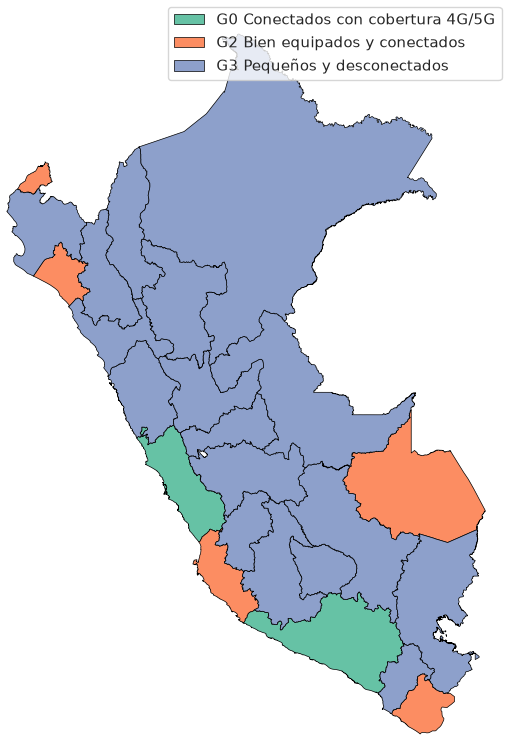
\includegraphics[height=3.9in]{figuras/mapa_perfil_predominante_recorte.png}
\hspace{0.06\textwidth}
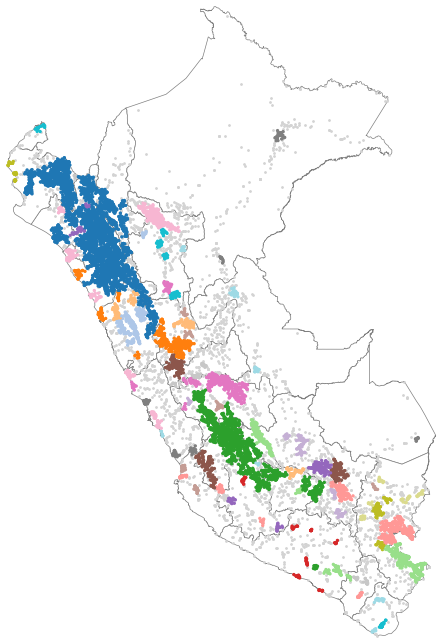
\includegraphics[height=3.9in]{figuras/mapa_focos_g3_recorte.png}
\caption{Izquierda: perfil con mayor porcentaje de locales en cada departamento. Derecha: focos espaciales de locales G3 (DBSCAN, 10 km); los puntos grises son ruido.}
\label{fig:mapas}
\end{figure*}

De los 42\,215 locales con perfil, 42\,214 tienen coordenadas válidas; 42\,205 caen dentro de una provincia y en 99,5~\% el departamento de la coordenada coincide con el declarado. Los perfiles no se distribuyen al azar (Fig.~\ref{fig:mapas}, izquierda). G0 predomina en Callao (99,0~\%), Lima (76,5~\%) y Arequipa (36,6~\%), con índices de concentración de 5,88, 4,54 y 2,17. G2 predomina en Ica, Lambayeque, Tacna, Tumbes y Madre de Dios. G3 predomina en los otros 17 departamentos, con los mayores porcentajes en Piura (49,1~\%) y Cajamarca (47,1~\%), frente a 31,4~\% nacional y 5,5~\% en Lima. G1 y G4 no predominan en ninguno, pero G1 llega a 28,8~\% en Huánuco y 27,2~\% en Puno, y G4 a 16,9~\% en Pasco.

Los 13\,241 locales de G3 forman 124 focos con 10 km y 2\,556 locales quedan como ruido (19,3~\%) (Fig.~\ref{fig:mapas}, derecha). El mayor foco reúne 4\,023 locales (30,4~\% de G3), sobre todo en Cajamarca, y le sigue uno de 1\,437 en Huancavelica. En Ucayali, Madre de Dios y Loreto entre 69,7~\% y 72,2~\% de los locales G3 son ruido, frente a 1,4~\% en Cajamarca. Esto sugiere desconexión continua en parte de la sierra norte y dispersa en la selva, aunque aún no se contrasta con la densidad del conjunto de locales.

\section{Problemas, limitaciones y trabajo pendiente}
\textbf{Problemas y limitaciones.}
\begin{itemize}
\item Ward solo pudo aplicarse a una muestra de 5\,000 locales por memoria; sus métricas no son estrictamente comparables con las de K-means.
\item DBSCAN sobre $Z_{df}$ no encuentra regiones densas separadas.
\item La cobertura móvil es distrital: todos los locales de un distrito comparten el valor, es lo que más separa a G0 y no asegura señal en el local.
\item Seis locales quedaron sin perfil por faltantes, y 24\,924 locales del censo no entran por no tener recursos registrados.
\item Los focos de G3 no se han contrastado con la densidad de todos los locales.
\end{itemize}

\textbf{Pendiente para el Hito 4.}
\begin{itemize}
\item Validar los grupos con área (urbano/rural) y gestión (pública/privada), que no entraron al clustering.
\item Detección de anomalías: locales atípicos dentro de su grupo.
\item Discusión global de los resultados, conclusiones y recomendaciones.
\end{itemize}

\begin{thebibliography}{00}
\bibitem{escale} Ministerio de Educación del Perú (MINEDU), Unidad de Estadística Educativa, ``Censo Educativo 2025: Padlocal, Ficha lineal del local, Recursos tecnológicos (P91) y Líneas de internet (P3230),'' ESCALE, 2025. [En línea]. Disponible: \url{https://escale.minedu.gob.pe}
\bibitem{osiptel} OSIPTEL, ``Porcentaje de cobertura móvil por centro poblado, empresa operadora y tecnología (2025-IV),'' Portal Nacional de Datos Abiertos, 2025. [En línea]. Disponible: \url{https://www.datosabiertos.gob.pe/dataset/porcentaje-de-cobertura-m%C3%B3vil-por-centro-poblado-empresa-operadora-y-tecnolog%C3%ADa}
\bibitem{lloyd} S. Lloyd, ``Least squares quantization in PCM,'' \emph{IEEE Trans. Inf. Theory}, vol. 28, no. 2, pp. 129--137, 1982.
\bibitem{jolliffe} I. T. Jolliffe y J. Cadima, ``Principal component analysis: a review and recent developments,'' \emph{Phil. Trans. R. Soc. A}, vol. 374, art. 20150202, 2016.
\bibitem{ward} J. H. Ward, ``Hierarchical grouping to optimize an objective function,'' \emph{J. Am. Stat. Assoc.}, vol. 58, no. 301, pp. 236--244, 1963.
\bibitem{ester} M. Ester, H.-P. Kriegel, J. Sander y X. Xu, ``A density-based algorithm for discovering clusters in large spatial databases with noise,'' en \emph{Proc. KDD}, 1996, pp. 226--231.
\bibitem{sklearn} F. Pedregosa \emph{et al.}, ``Scikit-learn: machine learning in Python,'' \emph{J. Mach. Learn. Res.}, vol. 12, pp. 2825--2830, 2011.
\bibitem{ign} Instituto Geográfico Nacional (IGN) y OCHA ROLAC, ``Peru: Subnational Administrative Boundaries (COD-AB), capa \url{per_admbnda_adm2_ign_20200714},'' Humanitarian Data Exchange, versión del 14/07/2020. [En línea]. Disponible: \url{https://data.humdata.org/dataset/cod-ab-per}
\bibitem{geopandas} M. Fleischmann \emph{et al.}, ``GeoPandas: fundamental data structures for vector spatial data in Python,'' \emph{Comput. Environ. Urban Syst.}, vol. 130, art. 102495, 2026.
\bibitem{rousseeuw} P. J. Rousseeuw, ``Silhouettes: a graphical aid to the interpretation and validation of cluster analysis,'' \emph{J. Comput. Appl. Math.}, vol. 20, pp. 53--65, 1987.
\bibitem{davies} D. L. Davies y D. W. Bouldin, ``A cluster separation measure,'' \emph{IEEE Trans. Pattern Anal. Mach. Intell.}, vol. PAMI-1, no. 2, pp. 224--227, 1979.
\end{thebibliography}

\end{document}
